\documentclass[11pt,notitlepage]{article}

\usepackage[comma,numbers,sort&compress]{natbib}
\usepackage{graphicx}
\usepackage{color}
\usepackage{soul}
\usepackage{amssymb}
\usepackage{amsbsy}
\usepackage{theorem}
\usepackage{xcolor}
\usepackage{fullpage}
\usepackage{amsmath}
\usepackage{bm}
\usepackage{empheq}
\usepackage{centernot}
\usepackage{mathtools}
\usepackage{stmaryrd}
\usepackage[margin=1cm]{caption}
\usepackage{algorithmic}
\usepackage{helvet}
\renewcommand{\familydefault}{\sfdefault}
\usepackage[affil-it]{authblk}
\usepackage[margin=1in]{geometry}
\usepackage{caption}
\usepackage{hyperref}
\captionsetup{font=small}

\usepackage{titlesec}

\titlespacing\section{0pt}{12pt plus 4pt minus 2pt}{0pt plus 2pt minus 2pt}
\titlespacing\subsection{0pt}{12pt plus 4pt minus 2pt}{0pt plus 2pt minus 2pt}
\titlespacing\subsubsection{0pt}{12pt plus 4pt minus 2pt}{0pt plus 2pt minus 2pt}
\setlength{\parindent}{0cm}
%\setlength{\parskip}{6pt}

\begin{document}

\thispagestyle{plain}
\pagenumbering{gobble}

\section{Summary vision statement}
Our proposal describes a knowledge engine in the spirit of Wolfram$|$Alpha \cite{Wolframalpha}: the user will query the system in natural language and the knowledge engine will parse the input, generate search strategies to fulfill the user question, execute a number of search strategies by traversing the relevant Knowledge Sources, and finally present results to the user. Similar to the highly successful Wolfram$|$Alpha, our knowledge engine will learn from repeated interactions with users to return the most relevant results. 

This system will be able to handle a variety of user queries, limited primarily by the content and variety of the NCATS translator knowledge beacons. In particular, our proposed knowledge engine will be able to process queries involving a number of biological entities and various interrogatives, with example questions including: \textit{How are disease X and Y related?}, \textit{How does variant X cause disease Y and protect against disease Z?}, \textit{What is the clinical outcome pathway for the treatment of disease X by drug Y?}, \textit{For all drugs used to treat disease X, which ones have the least well-studied clinical outcome pathway?}, etc.

This approach (detailed in the project description) addresses a number of limitations in the current NCATS reasoning tools (\url{https://github.com/NCATS-Tangerine/cq-notebooks}). In particular, the process of generating and executing search strategies will be automated, removing the need to write custom Python notebooks for each query type. Our system, based on a probabilistic Markovian architecture, will both learn from repeated user interaction and also dynamically incorporate uncertainty in all steps of the proposed process. Relevant knowledge sources will also be automatically identified, removing the need for users to be experts in the variety of biological databases available. Lastly, by returning a variety of ranked search strategies and answers, our knowledge engine will present a dossier of results allowing the user to appreciate subtlety and complexity when it naturally arises from an input query (eg. some questions have more than one ``correct'' answer). 

The team we have assembled to construct this knowledge engine possesses a wide range of applicable skills, from systems biology \cite{ramsey2010systems,hwang2005data1,hwang2005data2,de2004evolution}, natural language processing \cite{huang2012structured,huang2010dynamic,mi2008forest,huang2007forest}, mathematical algorithms for big data problems \cite{koslicki2014wgsquikr,holzinger2014entropy,koslicki2015coding,koslicki2013quikr,koslicki2017improving}, to database interaction and knowledge discover \cite{nandi2011guided,nandi2007effective,jagadish2007making,nandi2007assisted}. Individual components of this knowledge engine have been implemented for different applications (as detailed in the previous references) and similar paradigms are employed by a variety of previously implemented knowledge engines with high-profile examples including IBM's Watson \cite{ferrucci2010building} and the aforementioned Wolfram$|$Alpha \cite{Wolframalpha}.

Finally, the knowledge engine we propose will be built in a modular, extensible fashion allowing it to interact with new knowledge sources. Since we employ a Markov chain architecture to generate search strategies and a Dijkstra-like algorithm to execute them, new biological entities can easily be incorporated. The flexibility of this framework allows for quick integration of additional constraints and new query types with the advantage of not needing to re-train the entire system whenever a new extension is added (in contrast to deep learning/neural network architectures). 


%\begin{enumerate}
 %\item Core methodology:
%        \begin{enumerate}
%        \item  NLP parsing
%        \item  1st order probabilistic logic
%        \item modified Dijkstra
%        \item other probabilistic data analysis approaches?
%  		\end{enumerate}
 %\item Limitations addressed:
%        \begin{enumerate}
%        \item No incorporation of uncertainty in all steps of the process
%        \item inability to use natural language queries
%        \item inability to automate identification of relevant knowledge sources
%        \item inability to automate the selection of relevant queries
%        \end{enumerate}
% \item Expertise:
 %		\begin{enumerate}
%        \item Steve and Liang will have to put there expertise in here
%        Mine is: mathematical algorithms for fast approximate or exact analysis of big data problems (can give references)
%        \end{enumerate}
% \item Previous applications:
 %		\begin{enumerate}
%        \item Autonomous service robots (10.1177/0278364913481635),
%        \item IBM Watson is also based off of probabilistic evidence-based architecture (Magazine, A.I.~ ``The AI behind Watson -- the technical article.'' AI Magazine (2010).)
%        \item Suggested for use with precision oncology (10.1038/nrclinonc.2013.244)
%        \item Similar approaches in drug-target interaction prediction (10.1109/TCBB.2014.2325031)
%        \item Automatic question answering (10.1145/2396761.2398544)
%        \item Liang, more accurate previous applications?
%        \end{enumerate}
%\end{enumerate}

%\subsection{Limitations and bottlenecks in the current state of the art}

\newpage

\section{Project plan}
%\subsection{Overview of methodology to be used}
We propose a three-component system that will (i) process natural language user
queries, (ii) generate a dossier of ranked search strategies, and (iii) execute
the desired search strategies.
\subsection{Natural language processing}
\label{section:NLP}
A critical functionality of a reasoning engine is the ability to parse and
understand free-form user input. To facilitate this, we...  \textbf{Liang's NLP
  paragraph here} The NLP step will result in ... This representation of the
user query will be used by the reasoning engine to generate a dossier of search
strategies.

\begin{figure}[h!]
\centering
\begin{tabular}{c|c}
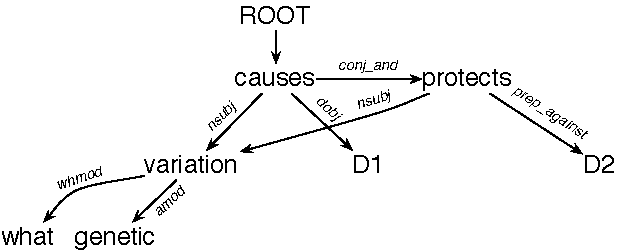
\includegraphics[width=0.4\textwidth]{stanford_parse}
&
\raisebox{2cm}{
\begin{tabular}{l}
cause (G?, D1)\\[0.5cm]
protect\_against (G?, D2)
\end{tabular}
}
\\
(a) syntactic parse &
(b) semantic parse
\end{tabular}
\caption{Natural language parsing of the input query
{\em``What genetic variant causes D1 and protects against D2?"}
where D1 and D2 are placeholders for two particular diseases.
(a) step 1, syntactic parsing: from query to Stanford dependencies.
(b) step 2, semantic parsing: from Stanford dependencies to first-order logic predicates.
}
\end{figure}

%an identification of relevant abstract terms (such as ``disease,'' ``pathway,'', ``molecule'' etc.) along with a desired connectives between them (such as ``offers protection against,'' ``is associated to'' etc.).
\subsection{Generate a dossier of search strategies}
\label{section:strategies}
Given a parsed natural language query as input, our Reasoning Engine will return
a {\em dossier\/} of possible {\em search strategies.\/} We define a search
strategy as a set of types of biological entities (these include genetic
variants, drugs, genes, molecules, pathways, diseases, diagnoses, phenotypes,
etc.) along with associated queries of Knowledge Sources to identify
relationships between pairs of those entities. Thus, each search strategy is a
connected, undirected graph in which each vertex corresponds to a type of
biological entity and each edge corresponds to a Knowledge Source that can
return tuples of associations for the entity types corresponding to the
respective vertices.  One or more terminal vertices in this graph correspond to
the entity types of the constants provided by the user's parsed natural language
query. To illustrate, we show the graphs for three simple search strategies that
the reasoning engine would include in the dossier for two user queries: {\em How
  are disease DX and disease DY connected?\/} (Fig.~\ref{fig:ugraph}a-b) and
{\em How does variant G cause disease DX and protect against disease DY?\/}
(Fig.~\ref{fig:ugraph}c).
\begin{figure}[h!]
  \begin{tabular}{ccc}
    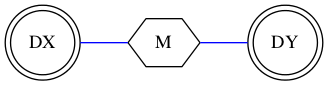
\includegraphics[width=1.2in]{net6.png} &
    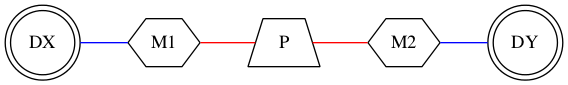
\includegraphics[width=2.2in]{net7.png} & 
    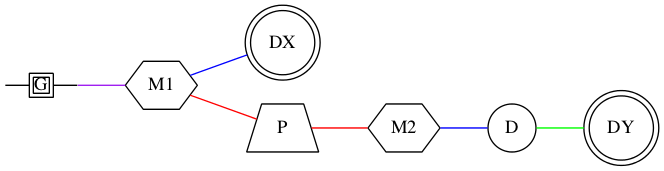
\includegraphics[width=2.5in]{net8.png} \\
                    {\bf (a)} & {\bf (b)} & {\bf (c)}
                    \end{tabular}
  \caption{Three example search strategies that might be included in dossiers
    returned by the reasoning engine: (a) and (b) are for a user query {\em How
      are disease DX and disease DY connected?\/}, which has two constants.
    Search strategy (c) is for a query {\em How does variant G cause disease DX
      and protect against disease DY?}  Double-shapes denote constants in the
    search strategy. Shape denotes an entity type (circle: disease; hexagon:
    molecule; trapezoid: pathway, box, variant). Internal vertex labels like
    ``M'' and ``P'' are placeholders representing the entity type, not a
    specific molecule. Edge color denotes the type of knowledge source to be
    searched (blue: disease-molecule association (e.g., DisGeNET, ClinVar); red:
    molecule-pathway association (e.g., Pathway Commons 2, BioCyc); green:
    disease-disease association (e..g, disease ontology, DNetDB); purple:
    variant-molecule association (e.g., ClinVar, BeFree). Arbitrarily complex
    search strategies can be created by chaining together additional possible
    entity-entity relationships, however, the reasoning engine will penalize
    possible search strategy graphs by the number of edges, in order to
    prioritize simpler search strategies.}
  \label{fig:ugraph}
\end{figure}

\subsubsection{How the reasoning engine will generate and prioritize search
  strategies}

In implementing the reasoning engine, we will use a Markov chain approach to
generate undirected graphs with the constant terms from the user's query as
terminal vertices in the graph. This approach enables the prioritization of
search strategies with fewer Knowledge Source lookups.  We will illustrate the
idea with a simple example, reprising the hypothetical user query {\em How are
  disease DX and disease DY connected?}. With two constants (i.e., terminal
vertices in the graph), the reasoning engine would generate graphs according to
the Markov process shown in Fig.~\ref{fig:mp}a).
\begin{figure}[h!]
  \begin{tabular}{cc}
    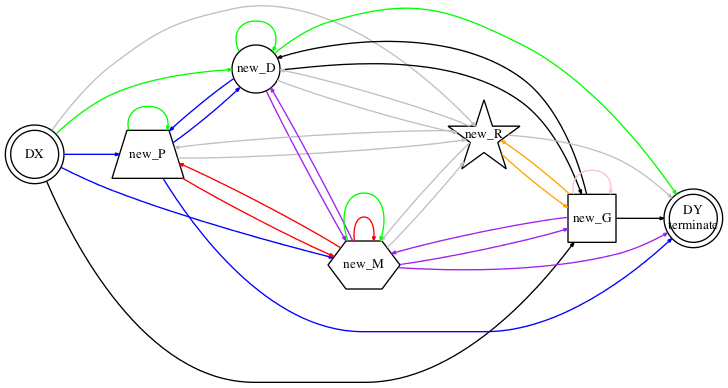
\includegraphics[width=3in]{markov1.png} &
    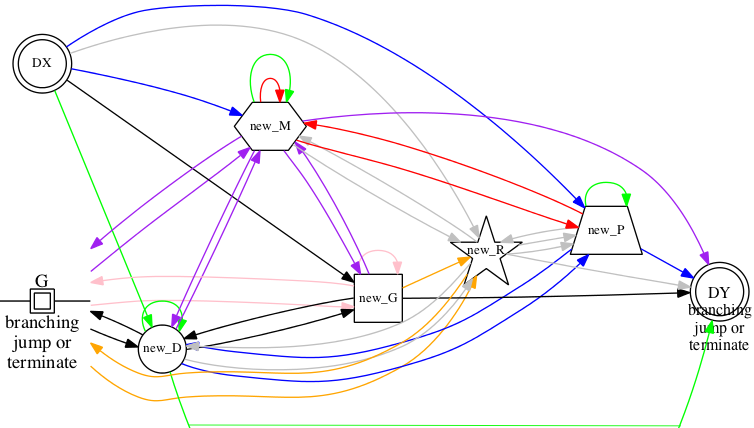
\includegraphics[width=3in]{markov2.png} \\
                    {\bf (a)} & {\bf (b)}
  \end{tabular}
  \caption{Markov chain transition digraphs for generating ranked query
    strategies for (a) an example two-constant natural-language query (diseases
    DX and DY) and (b) a three-constant natural-language query (variant G and
    diseases DX and DY). Double-circles and the double-box are the constants of
    the natural-language query (the two diseases and the variant, respectively).
    Colored arcs represent searches for entity-entity associations in various
    database sources [blue: disease-molecule association (e.g., DisGeNET,
      ClinVar); red: molecule-pathway association (e.g., Pathway Commons 2,
      BioCyc); green: disease-disease association (e..g, disease ontology,
      DNetDB); purple: variant-molecule association (e.g., ClinVar, BeFree);
      pink: variant-variant association (SNAP or IGSR); orange: drug-variant
      interaction (PharmGKB); is PharmGKB; black; variant-disease association
      (ClinVar, DisGeNET).] Each shape corresponds to a different type of
    biological entity (M, molecule; P, pathway, R, drug, G, variant, D,
    disease). In (b), if the Markov reaches a ``branching jump or terminate''
    state, the procedure is (i) add the indicated vertex to the undirected graph
    being constructed, (ii) remove the indicated vertex from the transition
    digraph, and (iii) select a non-leaf vertex in the undirected search
    strategy graph and begin extending a branch from that vertex.}
  \label{fig:mp}    
\end{figure}
Such digraphs will be constructed for each possible one-constant, two-constant,
and three-constant natural-language query. The digraph edges will have a
standard set of transition probabilities assigned. Each realization of the
Markov chain will generate a possible search strategy, i.e., an undirected graph
with the constant entities as terminal vertices; the Markov chain will also
assign a probability to each search strategy, penalizing excessively long chains
of Knowledge Source lookups and prioritizing the simplest strategies that can
connect the constant entities.

\subsubsection{Training of the Markov chain transition probabilities}
The transition probabilities (the weights of the
colored edges in Fig.~\ref{fig:mp}) will be determined empirically using a set
of 100 natural-language queries that we will assemble from template queries from
online NCATS-Translator resources and using biological mechanisms (and
successful search strategies for these queries that we will validate by hand)
for drug-variant interactions, variant-disease mechanisms, etc. We will select
transition probabilities that minimize the ranks of the 100 successful search
strategies for the 100 example queries, among the dossiers produced for these
queries (we will use the principal axes and eigenvalues of the Hessian to
prioritize important linear combinations of the log-probability weights to
fine-tune).

\subsubsection{A concrete example of how our reasoning engine would work}
Suppose a user wishes to find a common mechanism to identify a common mechanism
underlying the causal effect of variant rs334 for sickle-cell anemia and that
same variant's protective benefit against malaria. The natural-language query
has three constants, and one search strategy that would be ranked in the dossier
would be the one shown in Fig.~\ref{fig:ugraph}c. If executed against the
databases Pathway Commons (red), Disease Ontology (green), DisGeNET (blue), and
ClinVar (purple), the search strategy would return an explanatory mechanism, as
shown in Fig.~\ref{fig:malaria}, that is consistent with current knowledge of
the role of heme in cerebral malaria~\cite{Ferreira:2011ff}.
\begin{figure}[h!]
     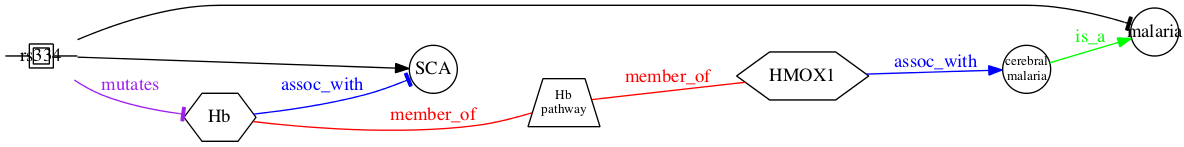
\includegraphics[width=6in]{net5.png} 
     \caption{Example of how the reasoning engine-returned search strategy of
       Fig.~\ref{fig:ugraph}c would find entity-entity associations across four
       databases that would suggest a common mechanism underlying the
       protective benefit of variant rs334 against malaria and the causal effect
       of rs334 for sickle-cell anemia. SCA, sickle-cell anemia; Hb,
       hemoglobin b; HMOX1, heme oxygenase 1.  Colors, database
       types (see Fig.~\ref{fig:mp}b).}
  \label{fig:malaria}
\end{figure}

\subsubsection{Beyond Markov chains---Markov Logic Networks}
We would additionally investigate the potential utility for constructing a
Markov Logic Network~\cite{Domingos:2012wi,domingos20071} that would
probabilistically represent possible connections between different types of
biological entities in different Knowledge Sources, as well as the nature of
those connections (e.g., inhibitory, causal, etc.). Such a model would represent
a generalization of the undirected graphical models that constitute the superset
of search strategies in our first reasoning engine prototype. As such, the use
of Markov Logic Networks could improve the ability to map parsed
natural-language queries to the search strategies that are most likely to yield
biologically relevant information.

%% Knowledge Sources, specific queries against those knowledge sources that will
%% return tuples of entities , and join operations connecting those entities. If
%% we conceptualize these entities as Without loss of generality, we will denote
%% identify relevant knowledge sources and construct appropriate queries in
%% order to answer user questions. This is accomplished by constructing a
%% network of \textit{schemas} and other metadata of Knowledge Sources (KS's)
%% which we call a \textit{schema network}. This representation will not be a
%% network of all biological interactions and entities contained in the KS's,
%% but rather it compactly and abstractly represents the categories of
%% information contained in the various Translator KS's as well as the
%% relationships between them. Hence, nodes are metadata entities (such as
%% \verb|disease| or \verb|pathway|) and edges between them are given by first
%% order logical statements (such as \verb|assoc_with(X,Y)|). Using the parsed
%% user input, our Reasoning Engine will identify paths in this schema network
%% that represent search strategies to answer the user query. These paths will
%% traverse one or more KS's metadata and hence will automatically identify the
%% relevant databases to query. To find such paths, we will implement a
%% reasoning engine based on the formalism of Tractable First-Order
%% Probabilistic Logic and its associated Tractable Markov Logic (TML) language
%% developed by \citet{Domingos:2012wi}. The identification of such paths is
%% equivalent to knowledge-based model construction, which is known to be
%% subsumed by Markov Logic \cite{domingos20071}.


%\subsubsection{Tractable Markov Logic} In keeping with the distributed nature
%of Translator's Knowledge Sources, the reasoning engine that will generate the
%dossier will operate on a Markov Logic Network learned from the {\em schemas\/}
%and other metdata of Knowledge Sources; it will not be a network of all
%biological interactions contained in the Knowledge Sources. The reasoning
%engine's input will be a data structure representing the parsed natural
%language query (see Sec.~\ref{sec:nlp}). The reasoning engine's output will be
%a {\em dossier,\/} i.e., a ranked list of {\em search strategies,\/} where a
%search strategy is a possible joining of result-sets from one or more queries
%of Translator Knowledge Sources (KS).


%% The goal will be to find paths in the schema network that describe common
%% mechanisms between the input diseases. One possible kind of path is a
%% (disease,disease) tuple representing ``is a subtype of'' relationships
%% (Fig.~\ref{fig:networks}b). This kind of relationship between diseases is
%% inferred from the metadata of the Gene Ontology database. An alternate path
%% consists of a undirected edges $\{$disease,disease$\}$ representing
%% disease-disease associations from the DisGeNET database
%% (Fig.~\ref{fig:networks}c). A more complicated path (traversing two different
%% databases) is given in Fig.~\ref{fig:networks}b) where (molecule,disease)
%% ``associated\_with'' tuples (from DisGeNET or Pharos) with (molecule,pathway)
%% tuples representing ``member\_of'' relationships from Pathway Commons. An
%% example of a {\em three}-database search strategy, for the same user query
%% (Fig.~\ref{fig:threedb}a) about a variant-to-two-diseases association, is shown
%% in Fig.~\ref{fig:threedb}b).


\subsection{Executing search strategies}
\label{section:Dijkstra}
After the search strategy (path through the schema network) is selected, we
employ a modified Dijkstra algorithm to find probable paths between source and
target node(s).  \textbf{Steve, Liang, insert description here}

%\subsubsection{Composition of the Markov Logic Network} We will use the
%Java-baesd (and open-source) NCATS-Tangerine Beacon Aggregator to obtain
%metadata (schemas and entity counts) from Knowledge Sources via RESTful queries
%leveraging the common Translator Knowledge Beacon Application Programming
%Interface (KBAPI).


%% Each of these possible paths identifies relevant KS's and represents a search
%% strategy: how to traverse these databases to answer the user query. A naive
%% approach to ranking these different search strategies would be to use a
%% combination of path length with edge weightings based on, say, prevalence of the
%% given diseases $D1$ and $D2$, strength of associations, etc. A more nuanced
%% approach is to utilize the TML language \citet{Domingos:2012wi} to rank the
%% search strategies in terms of how well they answer the user input. After the
%% user selects a desired search strategy (alternatively, the top ranked search
%% strategy is automatically utilized), the source and target nodes are grounded
%% with the particular biological entities contained in the user query. A modified
%% Dijkstra algorithm (Section \ref{section:Dijkstra}) is then used to execute the
%% query on the databases of interest to find paths between actual biological
%% entities.

%The schema network contains many different kinds of paths between a The schema
%network will contain various paths between the disease label and itself. For
%example, one such path is $D1$ ``is a``

%A simple strategy would be to search to obtain a list of (disease,disease)
%tuples representing ``is-a'' relationships from the Gene Ontology database
%(Fig.~\ref{fig:networks}b) where the edge would be assigned a weight in the
%Markov Logic Network based on the strength of evidence of this information type
%(either a fixed weight for the database, or with more information, the weight
%could be the ratio of prevalence of $D1$ to prevalence of $D2$). (We note that
%this search strategy would not be selected by the reasoning engine because the
%``is a'' relationship between two diseases is not consistent with the variant
%being protective against disease D2 and causal for disease D1). An alternative
%simple search strategy would be to load a list of {\em undirected\/}
%$\{$disease,disease$\}$ pairs representing disease-disease associations from
%the DisGeNET database (Fig.~\ref{fig:networks}c). An example of a {\em
%two}-database search strategy would be to join (molecule,disease)
%``associated\_with'' tuples (from DisGeNET or Pharos) with (molecule,pathway)
%tuples representing ``member\_of'' relationships from Pathway Commons
%(Fig.~\ref{fig:networks}d). An example of a {\em three}-database search
%strategy, for the same user query about a variant-to-two-diseases association
%(Fig.~\ref{fig:threedb}a), is shown in Fig.~\ref{fig:threedb}b.
%% \begin{figure}[h!]
%%   \begin{tabular}{ccc}
%%   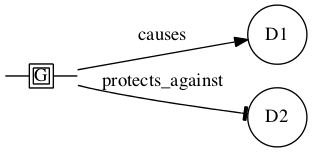
\includegraphics[width=1.4in]{baseproblem.png} &    
%%   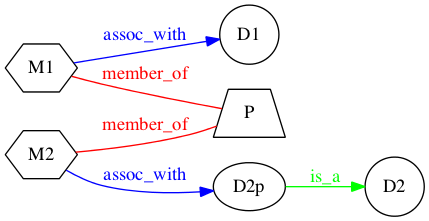
\includegraphics[width=2in]{net4.png} &
%%   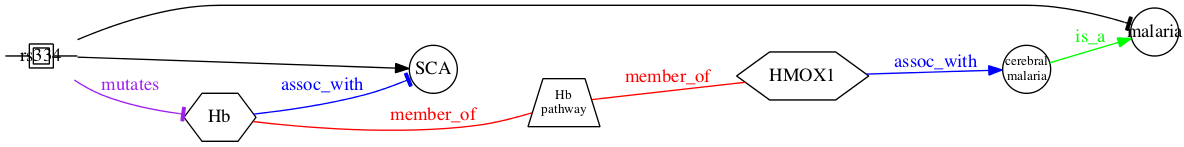
\includegraphics[width=2.5in]{net5.png} \\
%%                   {\bf (a) Query} & {\bf (b) Search Strategy 4} & {\bf (c) Search Result}
%%   \end{tabular}
%%   \caption{Example query predicate information (A); three-database example
%%     search strategy (B); matching search result for the specific query example
%%     G=rs334, D1=sicke-cell anemia (SCA) and D2=malaria (C). Edge color denotes
%%     the Knowledge Source to be searched (blue, DisGeNET; red, Pathway Commons;
%%     and green, Disease Ontology). Black edges denote the original query. Purple
%%     edge is the inferred interaction that explains the two black edges in light
%%     of the colored edges.}
%%   \label{fig:threedb}
%% \end{figure}
%% For example, assume that the variant G in this example query scenario is rs334,
%% a pleiotropic rare (MAF = 0.014\%) variant for which the homozygous minor allele
%% causes the blood disorder sickle-cell anemia (D1) and protects against malaria
%% (D2). A Dijkstra search on the three-database search strategy shown in
%% Fig.~\ref{fig:threedb}b) would yield a match indicating that a potential
%% explanation for the pleiotropy of rs334 is that it inhibits the hemoglobin
%% pathway, thus reducing circulating levels of free heme, which has been reported
%% to be protective in the case of cerebral malaria (a neurological complication of
%% malarial disease)~\cite{Ferreira:2011ff}.


\subsection{Anticipated functionality for the POC reasoning tool}
%\textit{Functionality for the reasoning tool proof-of-concept (due in Nov)}
For the two proof of concept project questions, the anticipated functionality includes (i) Allow the user to select from one of two questions: ``which genetic
  condition(s) protect(s) from a given disease $D$'' and ``what is the outcome
  pathway for drug $D$ and condition $C$''. The condition $C$ and/or drug $D$
  are specified by the user.
(ii) Pre-computed search strategies for these two questions will be implemented.
(iii) The modified Dijkstra algorithm will be implemented and will query the
  Knowledge Sources in real time (based on the user selected search query).

If funded, the Reasoning Engine we propose will allow for natural language input
(Section \ref{section:NLP}), automatic generation of search strategies (Section
\ref{section:strategies}) and will also utilize the Dijkstra algorithm of
Section \ref{section:Dijkstra}.

\subsection{Components of the proposed software stack}
The natural language processing will use the open source software \textbf{Liang: name and reference}. {\color{red} For the search strategy generation, there are a number of open source software
packages that implement Markov Logic Networks: Tuffy
\cite{DBLP:journals/pvldb/NiuRDS11}, Alchemy \cite{kok2006alchemy}, RockIt
\cite{noessner2013rockit}, and TheBeast \cite{riedel08improving}. We will
utilize Alchemy due to its robust implementation and continued development. }
The modified Dijkstra algorithm will be developed in-house and will be published
(in an open source fashion) on GitHub.

%\subsubsection{Natural language query analyzer} \label{sec:nlp} Should we use
%the Stanford CoreNLP with BioNLP shared task data? If so, which Python API
%should we use? (There are about a dozen of them).

\subsection{How proposed software will interact with Translator}
The Java-based (and open-source) NCATS-Tangerine Beacon Aggregator is used to obtain metadata (schemas and entity
counts) from Knowledge Sources via RESTful queries leveraging the common Translator Knowledge Beacon Application Programming Interface (KBAPI). This is used to set the architecture of the Markov chain. {\color{red} everything else including Dijkstra with API calls.}

%% \section{Background: Types of questions} \subsection{How does drug X induce
%% clinical outcome Y?}  \subsection{Why do variants that cause sicke-cell
%% anemia protect against malaria?}  \subsection{In people with variants found
%% in any of the 22 known FA genes, is there increasing incidence of apalastic
%% anemia (or other diseases)?}  \subsection{What venomous species have resulted
%% in drugs approved by the FDA?}  \subsection{What cellular processes in which
%% tissues are impacted in a patient-based EMR?}  \subsection{Why does ingestion
%% of GlcNAc ameliorate symptoms of ngly1 deficiency?}

%% \section{Background: Knowledge Sources}
%% \begin{description}
%% \item[EBI String]{Protein-protein interactions}
%% \end{description}

\section{Personnel}

\bibliographystyle{plainnat}
\bibliography{conclett}

\end{document}
